\documentclass{article}%
\usepackage[T1]{fontenc}%
\usepackage[utf8]{inputenc}%
\usepackage{lmodern}%
\usepackage{textcomp}%
\usepackage{lastpage}%
\usepackage[head=40pt,margin=0.5in,bottom=0.6in]{geometry}%
\usepackage{graphicx}%
%
\title{\textbf{Sujeto armado amenazó a periodistas que cubrían protesta frente al Ministerio de Educación}}%
\author{JOSÉ SILVA}%
\date{21/09/2018}%
%
\begin{document}%
\normalsize%
\maketitle%
\textbf{URL: }%
http://www.eluniversal.com/politica/21257/sujeto{-}armado{-}amenaza{-}a{-}periodistas{-}que{-}cubrian{-}protesta{-}frente{-}al{-}ministerio{-}de{-}educacion\newline%
%
\textbf{Periodico: }%
EU, %
ID: %
21257, %
Seccion: %
politica\newline%
%
\textbf{Palabras Claves: }%
NO\_TIENE\newline%
%
\textbf{Derecho: }%
1.3, %
Otros Derechos: %
, %
Sub Derechos: %
1.3.4\newline%
%
\textbf{EP: }%
SI\newline%
\newline%
%
\textbf{\textit{El reportero gráfico Luis Gonzalo Pérez aseguró que se defendió de una posible puñalada con un trípode de cámara}}%
\newline%
\newline%
%
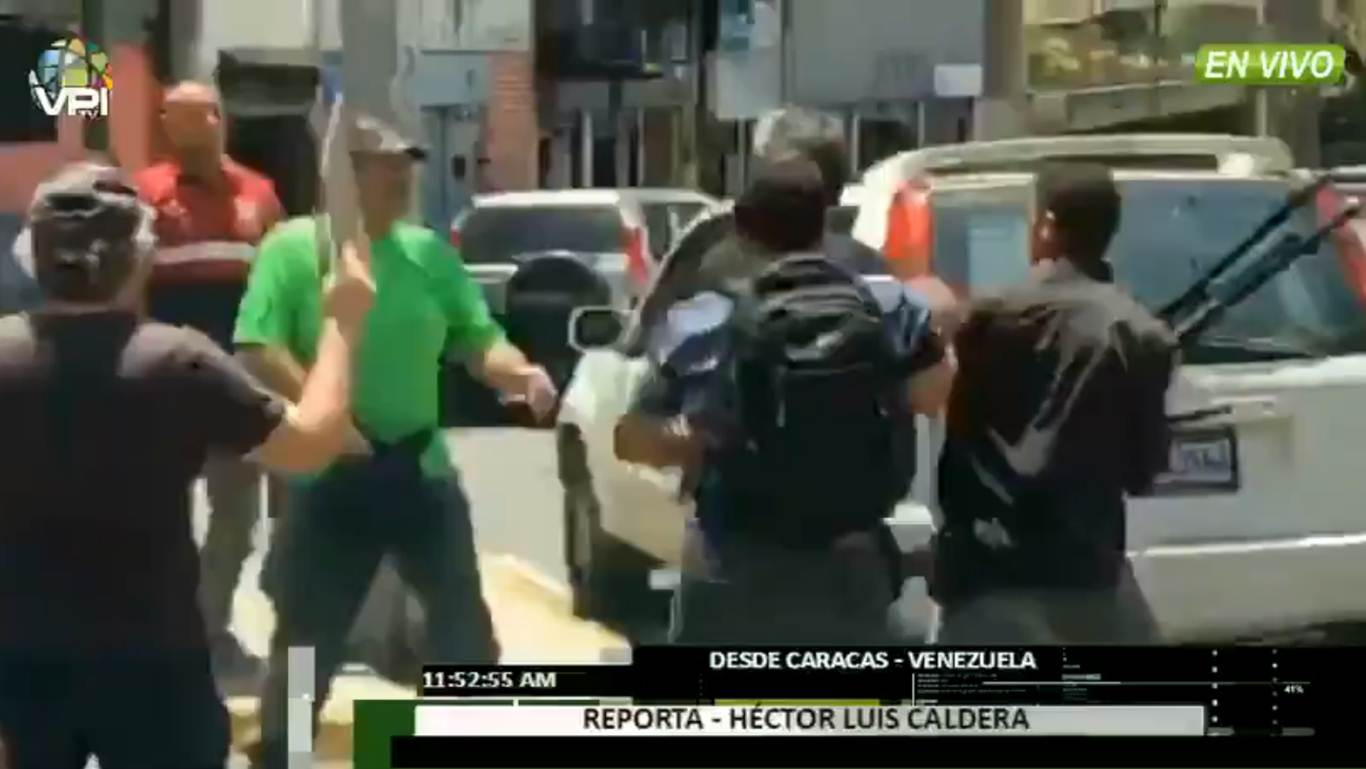
\includegraphics[width=300px]{180.jpg}%
\newline%
%
Caracas.{-} Este viernes un presunto colectivo amenazó con un arma blanca a un grupo de periodistas que cubrían una protesta frente a la sede del Ministerio de Educación.%
\newline%
%
El sujeto {-}que vestía con camisa verde, gorra y un bolso negro de lado{-} tenía un cuchillo en la mano derecha con el que intentó herir al reportero gráfico de NTN24, Luis Gonzalo Pérez, quien alegó que se defendió con un trípode de cámara.%
\newline%
%
Otros periodistas en conjunto con manifestantes rodearon al individuo para hacerle frente,~se pudo evidenciar en una transmisión del canal digital VPI.%
\newline%
%
Integrantes de la sociedad civil exigían, frente al Ministerio de Educación, mejores condiciones laborales para los docentes.%
\newline%
%
\end{document}